\section*{Exercises}

\bp Skipped.\ep 

\bp 
  Explain the error in the following "proof" that $2 = 1$. \\
  Let $x = y$. Then,

\begin{align}
x^2 &= xy \\
x^2 - y^2 &= xy - y^2 \\
(x+y)(x-y) &= y(x-y) \\
x+y &= y \\
2y &= y \\
2 &= 1
\end{align}
\ep 

\bs
  Since $x = y$, $x-y = 0$ and therefore, we cannot divided by $x-y$ in step $3$ to get $x+y = y$ from $(x+y)(x-y) = y(x-y)$. Thus, solved.
\es


\bp 
  Suppose that $m$ and $n$ are positive odd integers. Using $2 \times 1$ dominos,

  (a) Does there exist a perfect cover of the $m \times n$ chessboard?

  (b) If I remove 1 square from the $m \times n$ chessboard, will it have a perfect cover?
\ep 

\bs[a]
  In this case, there are $m \times n$ cells on the board which is an odd number. Since each domino covers only $2$ cells, the total number of cells covered will always be even.

  Hence, no perfect cover exists.
\es

\begin{scratch}[b]
  Let us take $3 \times 3$ chessboard. There are $9$ cells on the board. Without loss of generality, let us say there are $4$ white cells and $5$ black cells.

  Since a domino always covers $1$ white and $1$ black cell, the number of white and black cell must be equal for a perfect cover.

  Let us remove a black cell from the above chessboard. Now there are $4$ white cells and $4$ black cells.

  Checking all $5$ black squares for removal, we find that we have a cover in every case.
\end{scratch}

\bs[b]
  Let us assume that the board has $x$ white cells and $x+1$ black cells.
	Note: If it is not the case, we can always swap the colors and have the same setup.

	Since each domino must cover exactly $1$ white and $1$ black cell, we must remove a black cell to have a perfect cover.

	In this scenario, all the corners will have black cells since there are more black cells than white.

	Now, the question is, whether we can remove any black cell. 

	\begin{lemma}\label{even_chessboard}
		For every chessboard of size $m \times n$, there exists a cover if either $m$ or $n$ is even.
	\end{lemma}

	\begin{proof}
		Let us assume that $m$ is even. We can always turn the board if $n$ is even.

		For every column, we have an even number of cells in that column as $m$ is even. Hence, we can cover that column with dominos.

		Hence, proved.
	\end{proof}


	Let us say we removed a black cell from row $r$. Now, there are two cases:
	\bigbreak

	\underline{Case 1.} $r$ is odd.

	In this case, we can divide the remaining chessboard into $(r-1) \times n$ and $(m-r) \times n$ and cover them by Lemma \ref{even_chessboard}.
	
	\textbf{Note}: In case $r = 1$ or $r = m$, we only have one remaining part. The second part is empty and thus, requires no cover.
	
	Since the corners are black, the left most cell of every odd row must be black because the colors are alternating. That is, all the cells in first column and rows $1, 3, 5, ..., m$ must be black.

	Since $r$ is odd, the left most cell in it must be black.
	Thus, the columns containing black cells in row $r$ are odd, i.e., cells in columns $1, 3, 5, ..., n$ and row $r$ are black.

	Thus, if we remove any black cell from row $r$
	we will have divided the row into two even sized pieces, 
	which can be covered by the dominos by Lemma \ref{even_chessboard}.

	\bigbreak
	\underline{Case 2.} $r$ is even.

	In this case, we can take rows $r-1, r, r+1$ 
	and divide the remaining chess board in $(r-2) \times n$ and $(m-r-1) \times n$ 
	and cover them by Lemma \ref{even_chessboard}.

	Since $r$ is even, all the cells in row $r$ and columns $2, 4, 8, ..., n-1$ are black.
	
	Let us say we remove the cell in column $c$. Now, we can take column $c-1, c$ and $c+1$, 
	and divide the rest of cells into chess boards of sizes $(c-2)\times 3$ and $(n-c-1) \times 3$. Since $c$ is even, therefore, $c-2$ and $n-c-1$ are even as well.
	
	Thus, we can cover these boards using Lemma \ref{even_chessboard}.

	Now, for the remainig $3 \times 3$ board without its center, we can cover it like this:
	\bigbreak

	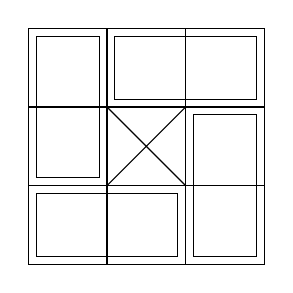
\begin{tikzpicture}
		\foreach \x in {0,1,2}
		\foreach \y in {0,1,2}
		{
			\draw (\x,\y) -- (\x+1,\y) -- (\x+1,\y+1) -- (\x,\y+1) -- (\x,\y);
		}

		\draw (1,1) -- (2,2) -- (1,2) -- (2,1);

		\draw (0.1,0.1) -- (1.9,0.1) -- (1.9,0.9) -- (0.1,0.9) -- (0.1,0.1);
		\draw (2.1,0.1) -- (2.9,0.1) -- (2.9, 1.9) -- (2.1,1.9) -- (2.1,0.1);
		\draw (2.9,2.1) -- (2.9,2.9) -- (1.1,2.9) -- (1.1,2.1) -- (2.9,2.1);
		\draw (0.1,1.1) -- (0.9,1.1) -- (0.9,2.9) -- (0.1,2.9) -- (0.1,1.1);
	\end{tikzpicture}

		Hence, proved.

\es

\bp 
  The game \textbf{Tetris} is played with five different shapes -- the five shapes that can be obtained by piecing together four squares.

\bigbreak

\resizebox{\textwidth}{!}{
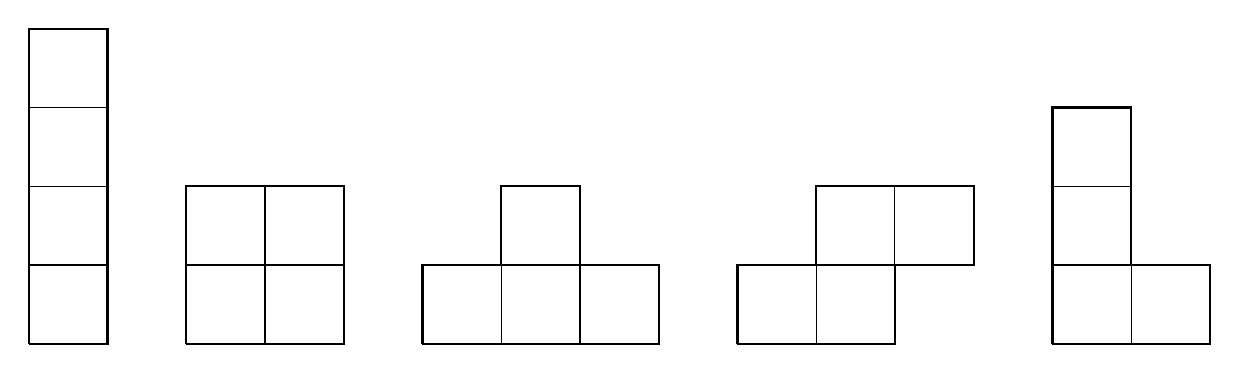
\begin{tikzpicture}
	\draw[thick] (0,0) -- (1,0) -- (1,4) -- (0,4) -- (0,0);
	\draw (0,1) -- (1,1);
	\draw (0,2) -- (1,2);
	\draw (0,3) -- (1,3);

	\draw[thick] (2,0) -- (4,0) -- (4,2) -- (2,2) -- (2,0);
	\draw (3,0) -- (3,2);
	\draw (2,1) -- (4,1);

	\draw[thick] (5,0) -- (8,0) -- (8,1) -- (7,1) -- (7,2) -- (6,2) -- (6,1) -- (5,1) -- (5,0);
	\draw (6,0) -- (6,1) -- (7,1) -- (7,0);

	\draw[thick] (9,0) -- (11,0) -- (11,1) -- (12,1) -- (12,2) -- (10,2) -- (10,1) -- (9,1) -- (9,0);
	\draw (10,0) -- (10,1) -- (11,1) -- (11,2);

	\draw[thick] (13,0) -- (13,3) -- (14,3) -- (14,1) -- (15,1) -- (15,0) -- (13,0);
	\draw (13,1) -- (14,1) -- (14,0);
	\draw (13,2) -- (14,2);
\end{tikzpicture}
}
\bigbreak

	For the questions below, we also allow these pieces to be "flipped over".

	(a) Is it possible to perfectly cover a $4 \times 5$ chessboard using each of these shapes exactly once? Prove that it is impossible, or show by example that it is possible.

	(b) Is it possible to perfectly cover an $8 \times 5$ chessboard using each of these shapes exactly twice? Prove that it is impossible, or show by example that it is possible.
\ep 

\begin{scratch}
	Let's color the chessboard in black and white. Here, we can see that all the shapes will cover $2$ black cells and $2$ white cells except the third shape.

	The third shape will cover either $3$ black and $1$ white cell or $1$ black and $3$ white cells.

	Therefore, if we use each shape exactly once, we will get either get a total of $11$ black and $9$ white cells or $9$ black and $11$ white cells.
\end{scratch}

\bs[a]
	Let's assume that it is possible to cover a $4 \times 5$ chessboard using these shapes exactly once.

	The chess board has exactly $10$ black and $10$ white cells in it. Each shape will take up exactly $2$ white and $2$ black cells except the third shape. 

	The third shape will either take up $3$ black and $1$ white cell or $3$ white or $1$ black cell. This is because all adjacent cells must be different color so if the center of the third shape is white, all the rest $3$ cells of that shape must be black and vice versa.

	Let's place each shape one by one. \\
	After placing the first shape, we will have $8$ black and $8$ white cells. \\
	After placing the second shape, we will have $6$ black and $6$ white cells. \\
	After placing the fourth shape, we will have $4$ black and $4$ white cells. \\
	After placing the fifth shape, we will have $2$ black and $2$ white cells.

	Now, we don't have enough white or black cells to place the third shape.
	This is a contradiction. Therefore, it is impossible to cover a $4 \times 5$ chessboard using each of these shapes exactly once.

	Hence, proved.
\es

\bs[b]
Giving an example:


\bigbreak
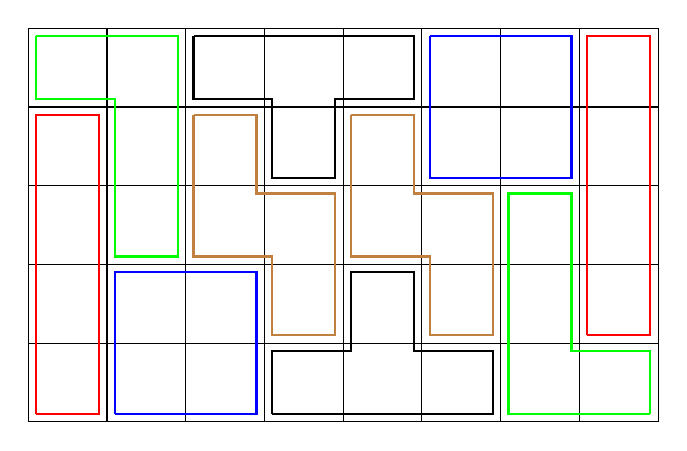
\begin{tikzpicture}
  \foreach \x in {0,1,2,3,4,5,6,7}
    \foreach \y in {0,1,2,3,4}
      {
        \draw (\x,\y) -- (\x+1,\y) -- (\x+1,\y+1) -- (\x,\y+1) -- (\x,\y);
			}

	% Long
	\draw[thick,red] (0.1,0.1) -- (0.1, 3.9) -- (0.9,3.9) -- (0.9,0.1) -- (0.1,0.1); 
	\draw[thick,red] (7.1,1.1) -- (7.1, 4.9) -- (7.9,4.9) -- (7.9,1.1) -- (7.1,1.1); 

	% Square
	\draw[thick,blue] (1.1,0.1) -- (1.1,1.9) -- (2.9,1.9) -- (2.9,0.1) -- (1.1,0.1);
	\draw[thick,blue] (5.1,4.9) -- (5.1,3.1) -- (6.9,3.1) -- (6.9,4.9) -- (5.1,4.9);

	% L-Piece
	\draw[thick,green] (0.1,4.9) -- (0.1,4.1) -- (1.1,4.1) -- (1.1,2.1) -- (1.9,2.1) -- (1.9, 4.9) -- (0.1,4.9);
	\draw[thick,green] (7.9,0.1) -- (6.1,0.1) -- (6.1, 2.9) -- (6.9, 2.9) -- (6.9, 0.9) -- (7.9, 0.9) -- (7.9, 0.1);

	% Z-Piece
	\draw[thick,brown] (2.1,3.9) -- (2.9,3.9) -- (2.9,2.9) -- (3.9,2.9) -- (3.9,1.1) -- (3.1,1.1) -- (3.1,2.1) -- (2.1,2.1) -- (2.1,3.9);
	\draw[thick,brown] (4.1,3.9) -- (4.9,3.9) -- (4.9,2.9) -- (5.9,2.9) -- (5.9,1.1) -- (5.1,1.1) -- (5.1,2.1) -- (4.1,2.1) -- (4.1,3.9);

	% T-Piece
	\draw[thick] (2.1,4.9) -- (2.1,4.1) -- (3.1,4.1) -- (3.1,3.1) -- (3.9,3.1) -- (3.9,4.1) -- (4.9,4.1) -- (4.9,4.9) -- (2.1,4.9);
	\draw[thick] (3.1,0.1) -- (3.1,0.9) -- (4.1,0.9) -- (4.1,1.9) -- (4.9,1.9) -- (4.9,0.9) -- (5.9,0.9) -- (5.9,0.1) -- (3.1,0.1);
\end{tikzpicture}

Hence, proved.
\es

\bp 
	If I remove two squares of different colors from an $8 \times 8$ chessboard, must the result have a perfect square?
\ep 

\bs
TODO
\es

\bp 
	If I remove four squares -- two white, two black -- from an $8 \times 8$ chessboard, must the result have a perfect cover?

	$\rightarrow$ If you believe a perfect cover exists, justify why.

	$\rightarrow$  If you belive a perfect cover does not need to exist, give an example of four squares that you could remove for which the result does not have a perfect cover.
\ep 

\bs
	TODO
\es

\bp 
	In chess, a \textbf{knight} is a piece that can move two squares vertically and one square horizontally, or two squares horizontall and one square vertically.

	A \textbf{knight} can legally move to any square provided there is not another piece on that same square.

	(a) Suppose there is a knight on every square of a $7 \times 7$ chessboard. Is it possible for every one of those knights to simultaneously make a legal move?

	(b) Suppose there is a knight on every square of a $8 \times 8$ chessboard. Is it possible for every one of those knights to simultaneously make a legal move?
\ep 


\bs[a]
Let us color the chessboard such that there are $24$ white squares and $25$ black squares without loss of generality.

In one move, a \textbf{knight} on a white square moves to a black square and vice-verse.

Since there are more black squares than white squares, we cannot move all the knight simultaneuosly such that all of them occupy different squares after the move by Principle \ref{pigeonhole}.
\es

\bs[b]
	In the first two rows of the $8 \times 8$ chessboard, there are $8$ white squares and $8$ black squares. We can pair them up like so:
\bigbreak

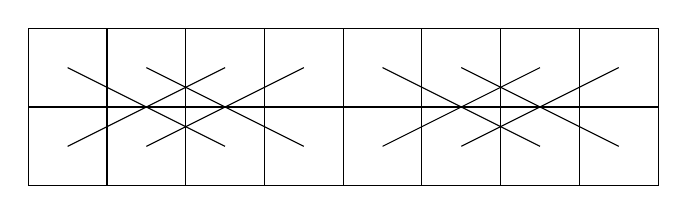
\begin{tikzpicture}
	\foreach \x in {0,1,2,3,4,5,6,7}
	\foreach \y in {0,1} {
		\draw (\x,\y) -- (\x+1,\y) -- (\x+1,\y+1) -- (\x,\y+1) -- (\x,\y);
	}
	\foreach \x in {0.5,1.5,4.5,5.5} {
		\draw (\x,1.5) -- (\x+2,0.5);
		\draw (\x+2,1.5) -- (\x,0.5);
	}
\end{tikzpicture}

This pattern can be repeat by every two rows of the board. And the knights in these places can swap positions.

Hence, proved.

\es

\bp 
	Prove that if one chooses $n+1$ numbers from $\{1, 2, 3, ..., 2n\}$, it is guaranteed that two of the numbers that they choose are consecutive.

	Also, before the proof, write 2 example for $n=3$, $n=4$ and $n=5$.
\ep 

\begin{scratch}
	For $n=3$, we can choose $4$ numbers from $\{1, 2, 3, 4, 5, 6\}$. Let them be $1, 3, 5, 6$. Here, $5$ and $6$ are consecutive.

	For $n=4$, we can choose $5$ numbers from $\{1, 2, 3, 4, 5, 6, 7, 8\}$. Let them be $1, 3, 5, 7, 8$. Here, $7$ and $8$ are consecutive.

	For $n=5$, we can choose $6$ numbers from $\{1, 2, 3, 4, 5, 6, 7, 8, 9, 10\}$. Let them be $1, 3, 5, 7, 9, 10$. Here, $9$ and $10$ are consecutive.
\end{scratch}

\bs
	Let us define the $n$ boxes numbered $1$ to $n$.
	For each selected $x$, if $x = 2k - 1$ or $x = 2k$, put it in the box $k$.

	Thus, box $k$ will only contain two numbers: $2 \cdot k - 1$ and $2 \cdot k$. Both these numbers are consecutive.

	Since there are $n+1$ selected numbers atleast two numbers must be in the same box by Principle \ref{pigeonhole} which implies that they are consecutive.

	Hence, proved.
\es

\bp 
	Assume that $n$ is a positive integer. Prove that if one selects any $n+1$ numbers from the set $\{1, 2, 3, ..., 2n\}$, then two of the selected numbers will sum to $2n+1$.
\ep 

\bs
	Let us define $n$ boxes numbered $1$ to $n$ such that box $i$ contains the numbers $i$ and $2n+1-i$.
	
	Thus, we will get boxes with numbers $(1, 2n), (2, 2n-1), ... (n, n+1)$. Note that the numbers in a box add up to $2n+1$.

	Now, since there are $n+1$ selected numbers atleast two numbers must be in the same box by Principle \ref{pigeonhole} which implies that they add up two $2n+1$.
\es


\bp 
	Explain in your own words what the general pigeonhole princple says.
\ep 

\bs
	If there are $n$ objects that are placed into $m$ boxes then there is atleast one box with atleast $\lfloor \frac{n}{m} \rfloor$ items in it.
\es


\bp 
	Prove that there are atleast two U.S. residents that have the same weight when rounded to the nearest \textbf{millionth} of a pound. 
\ep 

\bs
	A quick google search tells us that there are only $3.2$ million people over $300$ pounds in the U.S. and the population of the U.S. is $340$ million people.

	Thus, there are more than $330$ million people that weigh between $0$ and $300$ pounds.

	Let us create box for each weight with a millionth of a pound of precision. This will give us $300$ million boxes each denoting a weight with a precision of a millionth of a pound.

	Since there are more than $300$ million people in the U.S. who weigh between $0$ and $300$ pounds, by Principle \ref{pigeonhole}, we can conclude that there are atleast two people with the exact same weight when rounded to a millionth of a pound.
\es


\bp 
	Determine whetehr or not the pigeonhole principle guarantees that two students at your school have the exact three leter initials.
\ep 

\bs
	My school had $1000$ students in each year so a total of $4000$ students.

	There are $26 \cdot 26 \cdot 26 = 17576$ unique three letter initials.

	Therefore, the pigeonhole principle doesn't guarantee that two students at my school have the same three letter initial.
\es


\bp 
	Find your own real-world example of the pigeonhole principle.
\ep 

\bs
	There are $10,000$ engineers at my workplace. But there are only $366$ days in the year. 

	Therefore, atleast $\lfloor 10000/366 \rfloor = 27$ employees have the exact same joining anniversary.
\es

\begin{named}[Definition]
	Two integers $m$ and $n$ are said to be \emph{relatively prime} if there is no integer larger than $1$ which divides both $m$ and $n$.
\end{named}

This definition will be used in the following exercise.

\bp 
Prove that if one chooses $31$ numbers from the set $\{1,2,3,...,60\}$, 
that two of the numbers must be relatively prime.
\ep 

\bs
	We can use the same method as last one. We can create $30$ boxes where each box $k$ will contain the numbers $2k-1$ and $2k$. Thus, we will get boxes that contain the numbers $(1, 2), (3, 4), (5, 6) ..., (59, 60)$. 

	Here, it is obvious that both numbers in a box are relatively prime.

	Thus, putting $31$ selected numbers in these boxes, we will get atleast one box which has atleast two numbers.

	Therefore, there are two numbers that are relatively prime.

	Hence, proved.
\es

\bp 
	Assume that $n$ is a positive integer. Prove that if one chooses $n+1$ distince odd integers from $\{1, 2, 3, ..., 3n\}$, then atleast one of these numbers will divide another.

	Also, before your proof, check all possible selection of $4$ odd numbers from $\{1, 2, 3, ..., 9\}$, and for each selection locate two of the numbers for which one divdes the other.
\ep 

\begin{scratch}
	The following are the selections:
	\begin{itemize}
	\item $\{1, 3, 5, 7\}$ : $1$ divides $3$.
	\item $\{1, 3, 5, 9\}$ : $1$ divides $3$.
	\item $\{1, 3, 7, 9\}$ : $1$ divides $3$.
	\item $\{1, 5, 7, 9\}$ : $1$ divides $5$.
	\item $\{3, 5, 7, 9\}$ : $3$ divides $9$.
	\end{itemize}

	Since there are $\lfloor \frac{3n+1}{2} \rfloor$ odd numbers in the given setand we are choosing $n+1$, we need to put these numbers in $n$ boxes.

	Now, we want to choose $n$ boxes such that in each box the smaller number divides the larger number or the box has only one number.

	Let us say that for any selected number $x$, it can be written in the format $x = 3^k \cdot m$ where $k \geq 0$ and $m$ is not divisible by $3$.

	Now there are two cases:

	\underline{Case 1.} $n$ is odd.

	Now if $n$ is odd, The odd numbers are $\{1, 3, 5, 7, 9,..., 3n\}$. 
	There are $\frac{3n+1}{2}$ odd numebrs out of which $\frac{n+1}{2}$ are divisible by $3$. Now,
	$$\frac{3n+1}{2} - \frac{n+1}{2} = \frac{2n}{2} = n$$

	Thus, there are $n$ numbers not divisble by $3$.

	\underline{Case 2.} $n$ is even.

	Now, the odd numbers are $\{1, 3, 5, 7, 9, ..., 3n-1\}$.
	There are $\frac{3n}{2}$ odd numbers out of which $\frac{n}{2}$ are divisble by $3$. 

	Therefore, $n$ numbers are not divisble by $3$.

	Thus, if we create a box of $n$ numbers that are not divisble by $3$. 
	And place $n+1$ numbers in those boxes, such that if $x = 3^k \cdot m$ then put $x$ in box $m$.

	Then by Principle \ref{pigeonhole}, we will have atleast one box with two numbers in it. 

	Let us say $x_1 = 3^{k_1} \cdot m$ and $x_2 = 3^{k_2} \cdot m$ are both in box $m$ such that $k_1 < k_2$. Then,
	$$\frac{x_1}{x_2} = \frac{3^{k_1} \cdot m}{3^{k_2} \cdot m} = 3^{k_1-k_2}$$

	Since $k_1 > k_2$, we have shown that $x_2$ divides $x_1$.

	Thus, if we have two numbers in the same box, the smaller one divides the larger one.

	With that, let us move on to the solution.
\end{scratch}

\bs
There are two cases that we define:

\underline{Case 1.} $n$ is even.

In this case, the odd numbers are as follows: $\{1, 3, 5, ..., 3n-1\}$. 
By counting them, we can say that there are $\frac{3n}{2}$ odd numbers.

The numbers in the above set that are divisible by $3$ are as follows:
$\{3, 9, 15, ..., 3n-3\}$. This ends at $3n-3$ because $3n$ is even.
This set contains all the numbers from the set $\{1, 3, 5, ..., n-1\}$ multiplied by $3$.
Thus, by counting them, we get that there are $\frac{n}{2}$ numbers divisble by $3$.

Subtracting the first two counts, we get,
$$\frac{3n}{2} - \frac{n}{2} = \frac{2n}{2} = n$$
Thus, there are $n$ numbers in the set of odd numbers between $1$ to $3n$ such that they are not divisble by $3$.


\underline{Case 2.} $n$ is odd.

Since $n$ is odd $3n$ is also odd.

In this case, the odd numbers are as follows: $\{1, 3, 5, ..., 3n\}$. 
By counting them, we can say that there are $\frac{3n+1}{2}$ odd numbers.

The numbers in the above set that are divisible by $3$ are as follows:
$\{3, 9, 15, ..., 3n\}$.
This set contains all the numbers from the set $\{1, 3, 5, ..., n\}$ multiplied by $3$.
Thus, by counting them, we get that there are $\frac{n+1}{2}$ numbers divisble by $3$.

Subtracting the first two counts, we get,
$$\frac{3n+1}{2} - \frac{n+1}{2} = \frac{2n}{2} = n$$
Thus, there are $n$ numbers in the set of odd numbers between $1$ to $3n$ such that they are not divisble by $3$.


Hence, we have proved that for any $n$, the count of odd numbers not divisble by $3$ in the set $\{1, 2, 3, ..., 3n\}$ is $n$.

Now, let us take any number $x$ from the set of selected $n+1$ numbers. We can write $x$ in the form of $x = 3^k \cdot m$ where $k \geq 0$ and $m$ is an odd number which is not divisble by $3$.

Since $x$ is an odd number, therefore, all its factors must be odd as well. This implies that we can take out all the factors that are $3$ and will be left with an odd number $m$.

Now, let us define $n$ boxes for each odd number in $\{1, 2, 3, ..., 3n\}$ which is not divisible by $3$.

Now, we can put all $n+1$ numbers of the format $x = 3^k \cdot m$ in box $m$ since $m$ is not divisble by $3$.

By Principle \ref{pigeonhole}, since there are $n$ boxes and $n+1$ numbers, there must be a box $m$ with atleast two numbers.

Let us say that the numbers are $x_1 = 3^{k_1} \cdot m$ and $x_2 = 3^{k_2} \cdot m$ such that $k_1 > k_2$. ( Note: Since they are in the same box they have the same $m$. )

Now, we can show that,
$$\frac{x_1}{x_2} = \frac{3^{k_1} \cdot m}{3^{k_2} \cdot m} = 3^{k_1 - k_2}$$
Since $k_1 > k_2$, we can say that $x_1$ is divisble by $x_2$.

Hence, proved.

\es

\bp 
	Give an example of $100$ numbers from $\{1, 2, 3, ..., 200\}$ such that none of your selected numbers divides any of the others.
\ep 

\bs
	$$\{101,102,103,...,200\}$$
	In the above set, none of the numbers divide another since any multiple for a number greater than $100$ will be greater than $200$.
\es

\bp 
	Prove that any set of seven integers contains a pair whose sum or difference is divisible by $10$. 

	Also, give three examples of this before your proof. Have your sets contain a diverse set collection of integers.
\ep 

\begin{scratch}
	Examples:
	\begin{itemize}
		\item $\{ 1, 4, 5, 9, 19, 38, 42 \}$ : $38+42=80$ is divisble by $10$.
		\item $\{ 786, 124, 213, 468, 109, 309, 5876 \}$ : $786+124=910$ is divisble by $10$.
		\item $\{ 16, 27, 12, 70, 29, 45, 74 \}$ : $16+74=90$ is divisble by $10$.
	\end{itemize}
\end{scratch}

\bs
	Let us define $6$ boxes as follows: $(0), (1,9), (2,8), (3,7), (4,6), (5)$.

	Now, for each selected number we take its remainder when divided by $10$.
	For negative numbers, we can add $10$ until the remainder isn't positive.

	Now, since there are $7$ boxes atleast one box must have $2$ or more numbers by Principle \ref{pigeonhole}

	Now, we can show that we any box contains two or more numbers then those two numbers must either add or subtract to give a number divisible by $10$. We have the following cases for the box that contains two or more numbers:

	\underline{Case 1.} Box is $(0)$. \\
	Both numbers are divisble by $10$ so their sum is also divisible by $10$.

	\underline{Case 2.} Box is one of $(1,9),(2,8),(3,7),(4,6)$. \\
	If both numbers have the same remainder then their difference is divisble by $10$. \\
	If they have different remainders, then in all the cases, their remainders will add to make $10$, so their sum will be divisible by $10$.

	\underline{Case 3.} Box is $(5)$. \\
	Here, they both have a same remainder so their difference will be divisible by $10$.

	Hence, proved. 
\es

\bp 
	Prove that if one chooses any $19$ points from the interior of a $6 \times 4$ rectangle such that no three points are colinear, then there must exit four of these points which form a quadilateral of area at most $4$.
\ep 

\bs
	The area of the rectangle is $24$. Let us divide it into $6$ rectangles of are $4$ and dimensions $1 \times 4$.
	And let us define that if a point lies on a line that is shared between two rectangles 
	then that point is part of the upper rectangle that has a line as its edge.

	Since we are choosing $19$ points and we have $6$ rectangles that they can be placed in.
	By Principle \ref{pigeonhole} ( The Pigoenhole Principle ), there must be a rectangle with at least $4$ points.

	Since these four points lie inside the rectangle of an areaa $4$ and no three of them are colinear, therefore, they form a quadilateral and their area is at most $4$. 

	Hence, proved.
\es

\bp 
	Assume that $9$ points are choses from the right triangle with base and height of $2$. Assume that no three points are colinear. Prove that there exists three points which form a triangle whose area is less than $\frac{1}{2}$.
\ep 

\bs
	Here, the total area of the triangle is $2$.
	
	In this, the base is $2$, which can be divided into $4$ segments of $\frac{1}{2}$ each and we can connect them to the opposite vertex.

	Here, we have $4$ triangles with the same base and height. Note: Height is same because they will all have the same perpendicular from the opposite vertex.
	Thus, the area of these triangles is $\frac{1}{2}$.

	Now, selecting $9$ points that can be placed in these trianges, we will have atleast $1$ triangle with $3$ or more points by Principle \ref{pigeonhole}. 

	Since no $3$ points are colinear, these $3$ points form a triangle within another triangle of area $\frac{1}{2}$. Thus, the area of this triangle is less than or equal to $\frac{1}{2}$.

	The area is equal to $\frac{1}{2}$ only when the three points lie on the vertices of the triangle that they contain in.

\es


\bp 
	At a party, each person is acquainted with a certain number of others at the party and is a stranger to everyone else. Suppose there are $n \geq 2$ people at a party. Prove that atleast two people at this party have the same number of acquaintances at the party.

	Note: Being Acquaintances is symmetric. Every person is acquainted with atleast one person at the party.
\ep 

\bs
Since every person is acquainted with atleast one person at the party and no person can obviously be acquainted with themselves, therefore, the number of acquaintances of each person must lie between $1$ and $n-1$.

Let us create $n-1$ boxes and put each person in the box with the number of acquaintances that they have.

By Principle \ref{pigeonhole}, since there are $n$ people and $n-1$ boxes, there is atleast $1$ box with atleast $2$ people in it.

Therefore, there are atleast $2$ people at the party with the same number of acquaintances.
\es

\bp 
	(a) Determine the population of your hometown and how many non-balding people in your homwtown, if any, are guaranteed to have the same number of hairs on their head, according to the pigeonhole principle.

	(b) Determine, as best you can, the number of students who attended your high school while you were a senior. Then, determine how many of them, if any, are guaranteed to have the same birthday according to the pigeonhole principle.
\ep 

\bs Not Interested. Not Valueable. \es

\bp  
	The following conjectures are all false. Prove that they are false by finding a counter example to each.

(a) \underline{Conjecture 1:} If $x$ and $y$ are real numbers, then $|x+y| = |x| + |y|$.

\bs
	$x = 1, y = -1 \implies |x+y| = 0 \neq |x| + |y| = 2$
\es

(b) \underline{Conjecture 2:} If $x$ is a real number, then $x^2 < x^4$.

\bs
	$x = 0.1 \implies x^2 = 0.01, x^4 = 0.00001 \implies x^2 > x^4$
\es

(c) \underline{Conjecture 3:} Suppose $x$ and $y$ are real numbers. If $|x+y| = |x-y|$, then $y = 0$.

\bs
	$x = 0, y = 1, |x+y| = 1 = |x-y|$
\es
\ep 


\bp 
	Suppose you deal a pile of cards, face down, from a shuffled deck of cards ( only 13 cards of each suit ). How many must you deal out until you are guaranteed...

	(a) five of the same suit?

	\bs
		By Principle \ref{pigeonhole}, we have $n = 4$ boxes as suits. 
		We want atleast $k + 1 = 5 (\implies k = 4)$ in some box/suit.

		Thus, we must atleast have $kn+1 = 17$ cards.
	\es

	(b) two of the same rank?
	\bs
		By Principle \ref{pigeonhole}, we have $n = 13$ boxes as ranks. 
		We want atleast $k + 1 = 2 (\implies k = 1)$ in some box/rank.

		Thus, we must atleast have $kn+1 = 14$ cards.
	\es

	(c) three of the same rank?
	\bs
		By Principle \ref{pigeonhole}, we have $n = 13$ boxes as ranks. 
		We want atleast $k + 1 = 3 (\implies k = 2)$ in some box/rank.

		Thus, we must atleast have $kn+1 = 27$ cards.
	\es

	(d) four of the same rank?
	\bs
		By Principle \ref{pigeonhole}, we have $n = 13$ boxes as ranks. 
		We want atleast $k + 1 = 4 (\implies k = 3)$ in some box/rank.

		Thus, we must atleast have $kn+1 = 40$ cards.
	\es

	(e) two of one rank and three of another?
	\bs
		For $3$ cards of the same rank, we need atleast $40$ cards.
		
		In this case, we will already have another rank having two cards. 
		In the worst case, scenario, there will be $2$ cards in each rank/box for us to get to $40$ cards for $3$ cards in some rank/box.

		Thus, we need atleast $40$ cards.
	\es
\ep 


\bp 
	Determine the U.S. population at the time you are reading this.
	
	(a) Does the pigeonhole principle guarantee that $1$ million U.S.  residents have the same birthday?
	\bs
		There are $340$ million people in the U.S. There are $366$ days in the year.

		Thus, $n = 366$ and $k = 1000000$ which means we only need $366$ million and $1$ people ( $kn+1$ ) for atleast one day where $1$ million people have thier birthday.

		We clearly have more people than neeeded for this to be guaranteed. Hence, yes.
	\es


	(b) If the principle does not guarantee this, how many people are neede until that miltsone is reached? If the USA grows by $2$ million people per year, in what year will this occur?
	\bs The current population does guarantee it. \es
\ep 


\bp 
Imagine a friend gives you a deck of cards (a standard $52$-card deck) and lets you shuffle it a few times. They then ask you to slowly deal out the cards, one at a time, into a new pile on the table. The entire time the cards are face-down, so they have no idea which cards you are deailing.

At a certain point thisn procedure, they ask you to stop, and declare with confidence that the two stacks (hand and table) are in perfect balance.
They say the number of red cards in the stack in your hand is equal to the number of black cards in the stack on the table.
They let you count, and sure enough, they were correct.

There were no gimmicks in this procedure -- no trick cards or hidden cameras or outside help. How did your friend do it?
\ep 

\bs
	There are $23$ red and black cards each in a standard deck. 
	Let us divide the deck randomly into two decks of $23$ each and say that the first deck has $r$ red cards and $b$ black cards.

	Now, since there are $23$ red and black cards each, we have $23-r$ red and $23-b$ black cards in the second deck.

	Now, since each deck size is $23$, we know that 
	$$r + b = 23 \implies r = 23 - b$$
	Thus, number of red cards, $r$, in the first deck is the same as number of black cards, $23-b$, in the second deck.

	Thus, he only had to wait till I had dealt $23$ cards and stop me to make the claim.
\es

\bp 
	An alien creature has three legs, and on each o fhis three alien feet he wears an alien sock. Suppose he just washed $n$ triplets of alien socks ( $3n$ individual socks), and each triplet is a different color. If this alien pulls out his alien socks out of his alien dryer one-at-a-time, how many must he pull out to be guaranteed to have a matching triplet?
\ep 

\bs
	Here, we have $n$ colored triplets or boxes. We want atleast one box/color to have atleast $k+1 = 3$ socks which implies $k = 2$

	Thus, by Principle \ref{pigeonhole}, we need atleast $kn+1 = 2n+1$ socks.
\es

\bp 
	A magic square is an $n \times n$ matrix where teh sum of the entries in each row, column and diagonal equal the same value.

	An \textbf{anitmagic square} is an $n \times n$ matrix where each row, column and diagonal sums to a distinct value.

	Prove that, for every $n$, there does not exist an $n \times n$ antimagic square where each entry is $-1,0$ or $1$.
\ep 

\bs
	For each $n \times n$ matrix with entries $-1, 0$ or $1$, the sum of its rows, columns and diagonals can only be between $-n$ and $n$.

	Let us create $2n+1$ boxes labelled from $-n$ to $n$.

	Now, there are $n$ rows, $n$ columns and $2$ diagonals. Therefore, there are $2n+2$ sums that need to be distinct.

	But each sum must be placed in one of the $2n+1$ boxes. Therefore, by Principle \ref{pigeonhole}, there must be a box with two sums in it. This implies that the square cannot have distinct sum of rows, columns and diagonals.

	Thus, the antimagic square of size $n \times n$ with entries $-1,0$ or $1$ is not possible.
\es
